\documentclass[journal]{IEEEtran}
\usepackage[a5paper, margin=10mm]{geometry}
%\usepackage{lmodern} % Ensure lmodern is loaded for pdflatex
\usepackage{tfrupee} % Include tfrupee package


\setlength{\headheight}{1cm} % Set the height of the header box
\setlength{\headsep}{0mm}     % Set the distance between the header box and the top of the text


%\usepackage[a5paper, top=10mm, bottom=10mm, left=10mm, right=10mm]{geometry}

%
\setlength{\intextsep}{10pt} % Space between text and floats

\makeindex


\usepackage{cite}
\usepackage{amsmath,amssymb,amsfonts,amsthm}
\usepackage{algorithmic}
\usepackage{graphicx}
\usepackage{textcomp}
\usepackage{xcolor}
\usepackage{txfonts}
\usepackage{listings}
\usepackage{enumitem}
\usepackage{mathtools}
\usepackage{gensymb}
\usepackage{comment}
\usepackage[breaklinks=true]{hyperref}
\usepackage{tkz-euclide} 
\usepackage{listings}
\usepackage{multicol}
\usepackage{xparse}
\usepackage{gvv}
%\def\inputGnumericTable{}                                 
\usepackage[latin1]{inputenc}                                
\usepackage{color}                                            
\usepackage{array}                                            
\usepackage{longtable}                                       
\usepackage{calc}                                             
\usepackage{multirow}                                         
\usepackage{hhline}                                           
\usepackage{ifthen}                                               
\usepackage{lscape}
\usepackage{tabularx}
\usepackage{array}
\usepackage{float}
\usepackage{ar}
\usepackage[version=4]{mhchem}


\newtheorem{theorem}{Theorem}[section]
\newtheorem{problem}{Problem}
\newtheorem{proposition}{Proposition}[section]
\newtheorem{lemma}{Lemma}[section]
\newtheorem{corollary}[theorem]{Corollary}
\newtheorem{example}{Example}[section]
\newtheorem{definition}[problem]{Definition}
\newcommand{\BEQA}{\begin{eqnarray}}
\newcommand{\EEQA}{\end{eqnarray}}

\theoremstyle{remark}


\begin{document}
\bibliographystyle{IEEEtran}
\onecolumn

\title{12.41}
\author{INDHIRESH S- EE25BTECH11027}
\maketitle


\renewcommand{\thefigure}{\theenumi}
\renewcommand{\thetable}{\theenumi}

\textbf{Question}. The matrix $A =\myvec{4&3\\9&-2}$ has eigenvalues -5 and 7. The eigenvector(s) is/are
\begin{multicols}{2}
\begin{enumerate}
    \item $\myvec{1\\1}$
    \item $\myvec{3\\4}$
    \item $\myvec{2\\-6}$
    \item $\myvec{2\\8}$
\end{enumerate}
\end{multicols}
\textbf{Solution}:\\
Let us solve the given equation theoretically and then verify the solution computationally. \\
Given
\begin{align}
 \Vec{A} =\myvec{4&3\\9&-2}\;\;,\lambda_1=-5\;\;and\;\;\lambda_2=7
\end{align}
Now 

\begin{align}
  \Vec{A}\Vec{x}=\lambda\Vec{x}
\end{align}

\begin{align}
\myvec{\Vec{A}-\lambda\Vec{I}}\Vec{x}=0
\end{align}
Here $\Vec{x}$ is eigen vector.
\begin{align}
\myvec{\myvec{4&3\\9&-2}-\lambda\myvec{1&0\\0&1}}\Vec{x}=\myvec{0\\0}
\end{align}
For  $\lambda=-5$
\begin{align}
 \myvec{9&3\\9&3}\Vec{x}=\myvec{0\\0}
\end{align}
Let 
\begin{align}
   \Vec{x}=\myvec{a\\b}
\end{align}
By substituting Eq.6 in Eq.5 we get
\begin{align}
  9a=-3b
\end{align}

\begin{align}
  3a=-b
\end{align}
\begin{align}
    \Vec{x}=\myvec{a\\-3a}
\end{align}
\begin{align}
    \Vec{x}=a\myvec{1\\-3}
\end{align}
Where a is a scalar. So the eigen vector will be the scalar multiple of $\Vec{x}$.\\
For $a=2$
\begin{align}
    \Vec{x}=\myvec{2\\-6}
\end{align}
Option (3) is correct

For  $\lambda=7$
\begin{align}
 \myvec{-3&3\\9&-9}\Vec{x}=\myvec{0\\0}
\end{align}

By substituting Eq.6 in Eq.11 we get
\begin{align}
    a=b
\end{align}
\begin{align}
    \Vec{x}=\myvec{a\\a}
\end{align}
\begin{align}
    \Vec{x}=a\myvec{1\\1}
\end{align}
Where a is a scalar. So the eigen vector will be the scalar multiple of $\Vec{x}$.\\
For $a=1$
\begin{align}
    \Vec{x}=\myvec{1\\1}
\end{align}
Option (1) is also correct



From the figure it is clearly verified that the theoretical solution matches with the computational solution.\\
\begin{figure}[h]
    \centering
    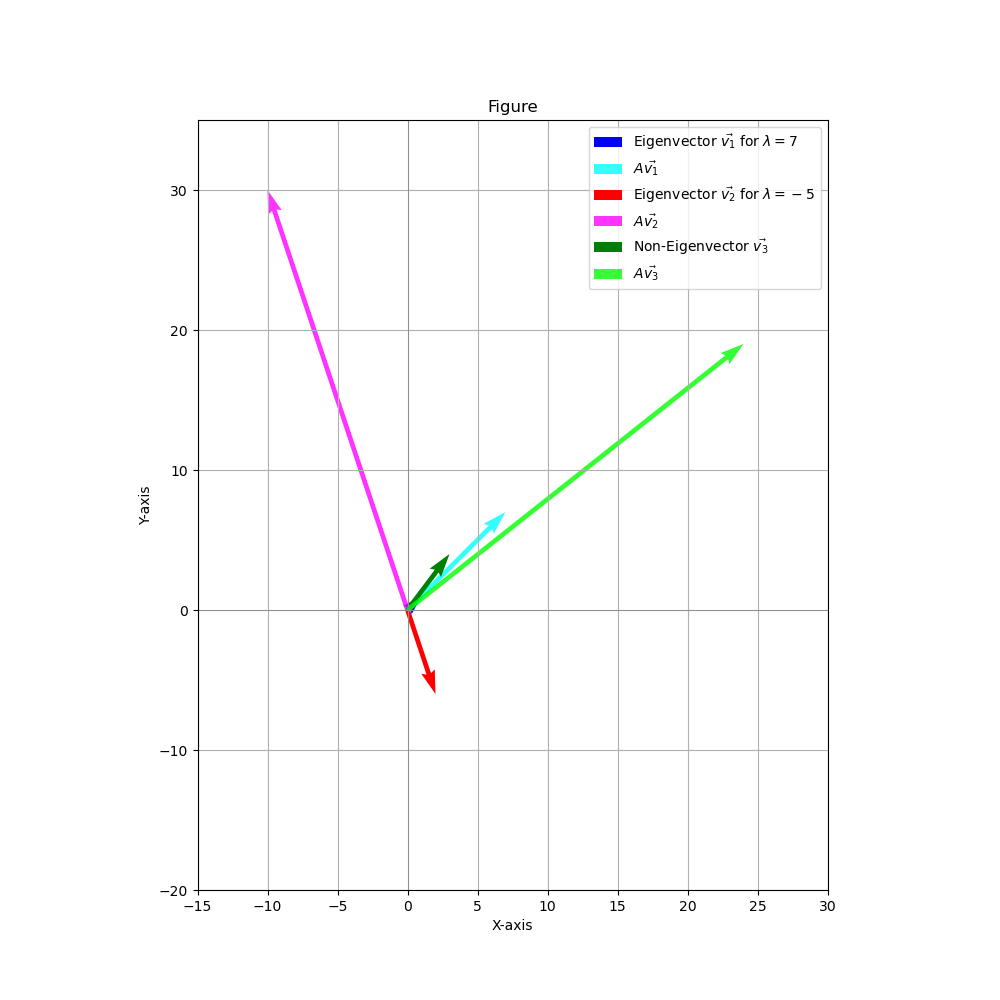
\includegraphics[height=0.5\textheight, keepaspectratio]{figs/figure1.png}
    \label{figure_1}
\end{figure}

\end{document}